\documentclass{beamer}
\usepackage{multicol}
\usepackage{common/lstlinebgrd}
\usepackage{common/beamerthemeUpceFei}
\usepackage{common/code}

\usepackage{amssymb}% http://ctan.org/pkg/amssymb
\usepackage{pifont}% http://ctan.org/pkg/pifont
\newcommand{\cmark}{\ding{51}}%
\newcommand{\xmark}{\ding{55}}%


\graphicspath{{images/}} % Location of the graphics files


\newcommand\fullscreenFrameImage[2][height=\paperheight]{%
\begin{frame}[plain]
\makebox[\linewidth][c]{%
  \begin{minipage}{\dimexpr\textwidth+2cm\relax}
  \raggedright
  \colorbox{white} {
    \makebox[\linewidth]{\includegraphics[#1]{#2}}
    }
  \end{minipage}%
  }%
  \end{frame}
}

\author{Petr Filip}
\title{Programování internetových aplikací - CSS}
\institute{Univerzita Pardubice}
%\date{September 18, 2007}

\newcommand{\h}[1]{H^{(1)}_{#1}}


\usepackage{amsmath}
\begin{document}



\maketitle


\section{VCS \& Github.com} 

\begin{frame}{VCS \& Github.com}
\begin{itemize}
	\item pro verzování zdrojového kódu
	\item pro efektivní práci v týmu
	\item \textbf{pro odevzádávání Vašich prací}
\end{itemize}

\begin{itemize}
	\item Jak začít?
	\item \url{https://youtube.com/watch?v=Vxy5b5KpN7E}
\end{itemize}

\begin{itemize}
	\item Celá řada GIT klientů:
	\begin{itemize}
		\item integrace s IntelliJ Idea (jetbrains)
		\item VCS > Import into version control > Share project on github
		\item Github \url{https://desktop.github.com/} (zatím ne Unix)		
		\item TortoiseGit		
	\end{itemize}
\end{itemize}
\end{frame}
  
\section{Kaskádové styly}
  
\begin{frame}{Kaskádové styly}
	Cascading Style Sheet (kaskádové styly) je stylový
jazyk, který se používá pro popis vzhledu a
formátování dokumentů napsaných značkovacím
jazykem.

Nejčastěji se CSS používá pro grafickou prezentaci
HTML stránek. Další použití lze nalézt např. u XML.

Podpora nových CSS vlastností je v prohlížečích
diskutabilní. U některých vlastností je i rozdíl v
samotné implementaci (stejná vlastnost se v
různých prohlížečích chová odlišně).
\end{frame}  

\begin{frame}{Syntaxe}

Styl se skládá z pravidel pro jednotlivé elementy,
které mají být formátovány. Každé takové pravidlo
má dvě části, selektor (název elementu, pro který
má toto pravidlo platit) a deklaraci (co pro něj má
platit). V deklaraci určujeme vlastnost a její hodnotu,
deklarace je uzavřena do složených závorek.

SELEKTOR \{vlastnost: hodnota\}

	
\end{frame}

\begin{frame}[fragile, shrink=0]{Ukázka použití CSS}
\begin{itemize}
	\item HTML:
\end{itemize}
\begin{lstlisting}[language=HTML]
<div>My text</div>
\end{lstlisting}

\begin{itemize}
	\item CSS:
\end{itemize}
\begin{lstlisting}[language=CSS]
div {
    color: red;
}
\end{lstlisting}
\begin{itemize}
	\item Výsledek:
\end{itemize}

\textcolor{red}{My text}
 
\end{frame}

\begin{frame}[fragile, shrink=0]{Možnosti použití CSS}

\begin{itemize}
	\item Přímý styl
\end{itemize}
\begin{lstlisting}[language=HTML]
<div style="color:red">My text</div>
\end{lstlisting}

\begin{itemize}
	\item Stylopis v hlavičce
\end{itemize}
\begin{lstlisting}[language=HTML]
<style> 
	div { color: red; }
</style>
\end{lstlisting}

\begin{itemize}
	\item Externí soubor
\end{itemize}
\begin{lstlisting}[language=HTML]
<link href="styly.css" 
type="text/css" 
rel="stylesheet">
\end{lstlisting}
\end{frame}

\section{W3SCHOOLS - CSS}

\section{Projektové cvičení}

\begin{frame}[fragile, shrink=0]{Projektové cvičení - CSS footer}
View > Quick documentation in IntelliJ Idea

Ctrl+Shift+Space
\end{frame}

\begin{frame}{Rozložení webové stránky}
  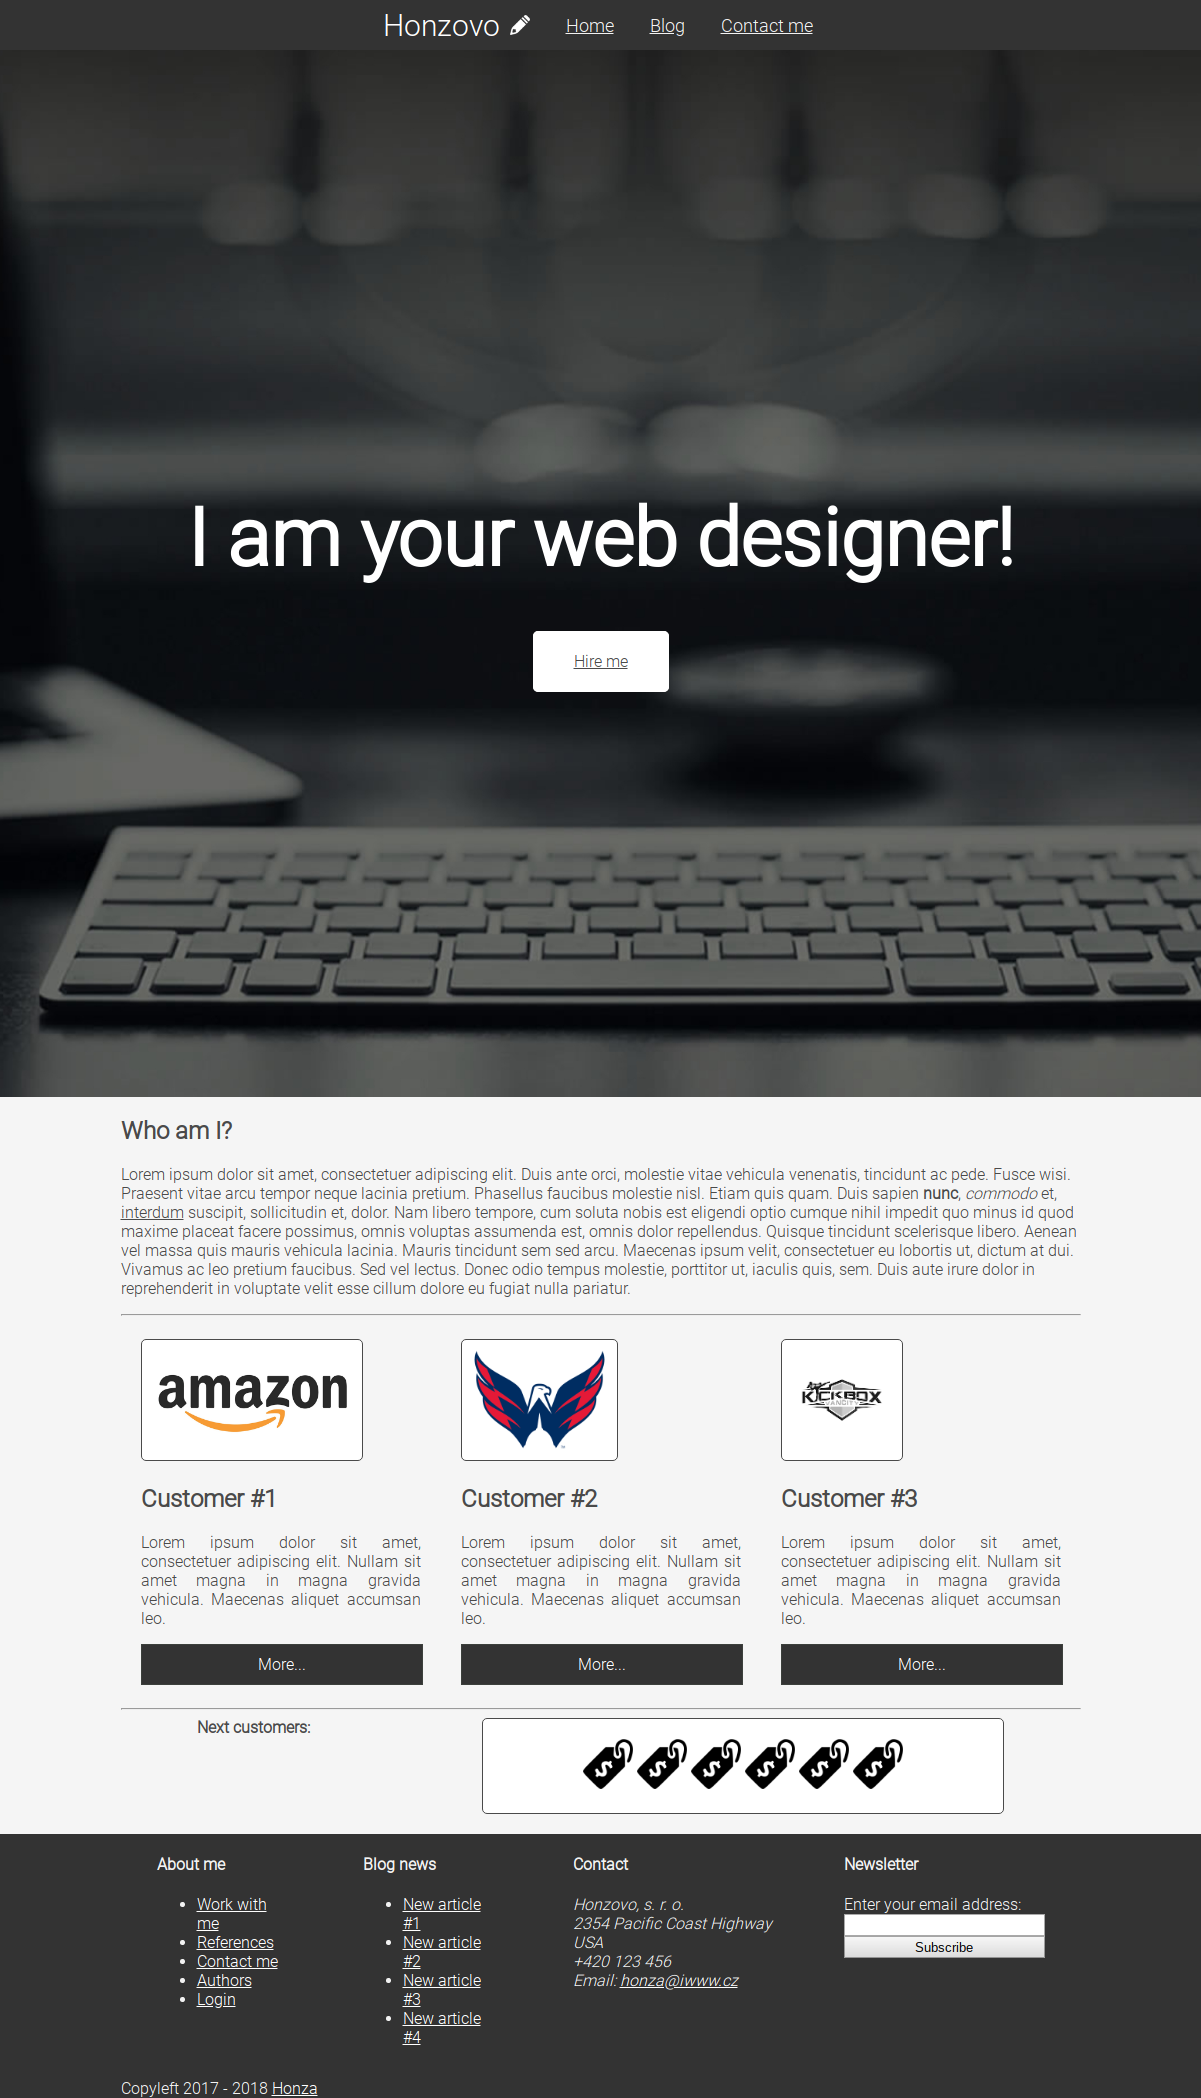
\includegraphics[scale=0.1]{project}
\end{frame}


\begin{frame}[fragile, shrink=0]{Projektové cvičení - úprava hlavičky}

\begin{lstlisting}[language=HTML]
<!DOCTYPE html>
<html lang="en">
<head>
    <meta charset="UTF-8">
    <link rel="stylesheet" type="text/css" 
     href="./css/layout.css">
    <title>Honzovo | Web developer</title>
</head>
\end{lstlisting}
	
\end{frame}


\begin{frame}[fragile, shrink=0]{Projektové cvičení - úpravy HTML}

\begin{lstlisting}[language=HTML]
<main>
    <div class="center-wrapper">
\end{lstlisting}
	
\noindent\rule{\textwidth}{1pt}


\begin{lstlisting}[language=HTML]
<hr/>
<div class="flex-wrap">
  <div class="card">
    <img src="../../../images/customerOne.jpg"/>
\end{lstlisting}

\noindent\rule{\textwidth}{1pt}

\begin{lstlisting}[language=HTML]
<div class="flex-wrap">
   <strong>Next customers:</strong>
\end{lstlisting}

\noindent\rule{\textwidth}{1pt}

\begin{lstlisting}[language=HTML]
<footer>
    <div class="full-width-wrapper">
        <div class="flex-wrap">
\end{lstlisting}
	
\end{frame}

\begin{frame}[fragile, shrink=0]{Projektové cvičení - CSS top level}
\url{https://www.w3schools.com/css/css3_flexbox.asp}
\begin{lstlisting}[language=CSS]
body {
    margin: 0;
    background-color: #F5F5F5;
    font-family: 'Roboto', sans-serif;
    font-size: 16px;
    color: #4a4a4a;
}

\end{lstlisting}
	
\end{frame}


\begin{frame}[fragile, shrink=0]{Projektové cvičení - CSS header}

\begin{lstlisting}[language=CSS]
body {
            margin: 0;
            background-color: #F5F5F5;
            font-family: 'Roboto', sans-serif;
            font-size: 16px;
            color: #4a4a4a;
        }
        header {
            top: 0;
            width: 100%;
            z-index: 1;
            display: flex;
            align-items: center;
            justify-content: center;
            background-color: #333;
        }

        header nav a {
            display: inline-block;
            color: #f2f2f2;
            text-align: center;
            padding: 14px 16px;
            text-decoration: underline;
            font-size: 18px;
        }

        header nav a:hover {
            background-color: white;
            color: black;
        }
\end{lstlisting}
	
\end{frame}


\begin{frame}[fragile, shrink=0]{Projektové cvičení - CSS \#header}

\begin{lstlisting}[language=CSS]
#header-web-title {
    color: white;
    font-size: 30px;
    margin: 10px;
}

#header-logo {
    width: 20px;
    margin-right: 20px;
}
\end{lstlisting}
	
\end{frame}


\begin{frame}[fragile, shrink=30]{Projektové cvičení - CSS \#hero}

\begin{lstlisting}[language=CSS]
#hero {
    height: 100%;
    background: url("hero.jpg") no-repeat center;
    background-size: cover;
    position: relative;
    text-align: center;
    display: flex;
    align-items: center;
    justify-content: center;
    color: white;
}

#hero h1 {
    font-size: 3em;
}

#hero a {
    padding: 20px 40px;
    background-color: white;
    border-radius: 5px;
    color: #4a4a4a;
    border: 1px solid white;
    transition: 1s;
}

#hero a:hover {
    background-color: black;
    color: white;
    border: 1px solid white;
}
\end{lstlisting}

\end{frame}


\begin{frame}[fragile, shrink=0]{Projektové cvičení - CSS footer}

\begin{lstlisting}[language=HTML]
footer {
            margin-top: 20px;
            min-height:200px;
            left: 0;
            display: flex;
            bottom: 0;
            width: 100%;
            background-color: #333;
            color: #f2f2f2;
            align-items: center;
            justify-content: center;
        }
        footer div {
            width: 33%;
        }
        footer a {
            color: white;
        }
\end{lstlisting}
	
\end{frame}






%\section{Opakování}



%\begin{frame}{Třída a identifikátor I.}
	
%\end{frame}

%\begin{frame}{Třída a identifikátor II.}
	
%\end{frame}
  
%\begin{frame}{Délkové jednotky}
	
%\end{frame}

  
%\begin{frame}{Barvy}
	
%\end{frame}


\section{Opakování}

\begin{frame}{CSS selektory I.}

\resizebox{\linewidth}{!}{%
\begin{tabular}{|l|l|l|}
	\hline
	\multicolumn{1}{|c|}{\textbf{Selector}} & \multicolumn{1}{c|}{\textbf{Example}} & \multicolumn{1}{c|}{\textbf{Example description}} \\ \hline
.class & .intro & Selects all elements with class="intro" \\ \hline
\#id & \#firstname & Selects the element with id="firstname" \\ \hline
* & * & Selects all elements \\ \hline
element & p & Selects all <p> elements \\ \hline
element,element & div, p & Selects all <div> elements and all <p> elements \\ \hline
element element & div p & Selects all <p> elements inside <div> elements \\ \hline
element>element & div > p & Selects all <p> elements where the parent is a <div> element \\ \hline
element+element & div + p & Selects all <p> elements that are placed immediately after <div> elements \\ \hline
element1\char`\~ element2 & p\char`\~ul & Selects every <ul> element that are preceded by a <p> element \\ \hline
[attribute] & [target] & Selects all elements with a target attribute \\ \hline
[attribute=value] & [target=\_blank] & Selects all elements with target="\_blank" \\ \hline
[attribute\char`\~=value] & [title\char`\~=flower] & Selects all elements with a title attribute containing the word "flower" \\ \hline
\end{tabular}
}


\begin{itemize}
	\item \url{http://jecas.cz/css-selektory}
	\item \url{https://w3schools.com/cssref/css_selectors.asp}
	\item \url{https://jakpsatweb.cz/css/css-vlastnosti-hodnoty-prehled.html\#selektory}
\end{itemize}
\end{frame}

\begin{frame}{CSS selektory II.}


\begin{tabular}{|l|l|}
\hline
\textbf{Selector} 		& \textbf{description} \\  \hline
	E:link 				& ještě nenavštívený odkaz\\  \hline
	E:visited 			& již navštívený odkaz\\  \hline
	E:active 			& aktivovaný odkaz\\  \hline
	E:hover			 	& zaměřený odkaz (myší)\\  \hline
	E:empty 			& element, který nemá potomky\\  \hline
	E:first-child  		& první potomek elementu E\\  \hline
	E:last-child  		& poslední potomek elementu E\\  \hline
	E::first-line 		& první řádka elementu E\\  \hline
	E::first-letter 	& první písmeno elementu E\\  \hline

\end{tabular}


\end{frame}



\begin{frame}{CSS display}

\begin{itemize}
	\item Základní způsoby zobrazení prvku: 
	\begin{itemize}
		\item inline
		\item inline-block
		\item block
		\item none
	\end{itemize}
\end{itemize}

\resizebox{\linewidth}{!}{%
\begin{tabular}{|l|l|l|l|}
\hline
\multicolumn{1}{|c|}{\textbf{\textit{Behavior}}} & \multicolumn{1}{c|}{\textbf{inline}} & \multicolumn{1}{c|}{\textbf{inline-block}} & \multicolumn{1}{c|}{\textbf{block}} \\ \hline
Respects left/right padding & 	\cmark & \cmark & \cmark \\ \hline
Respects left/right margin & 	\cmark & \cmark & \cmark \\ \hline
Respects top/bottom padding & 	\cmark & \cmark & \cmark \\ \hline
Respects top/bottom margin & 	\xmark & \cmark & \cmark \\ \hline
Default width is width of its container (not width of its contents) & \xmark & \xmark & \cmark \\ \hline
Forces a line break (does not allow elements to sit beside it) & \xmark & \xmark & \cmark \\ \hline
Respects height/width when specified & \xmark & \cmark & \cmark \\ \hline
\end{tabular}%
}

\begin{itemize}
	\item \url{https://codepen.io/petrfilip/pen/ReLxOJ}
	\item \url{https://jakpsatweb.cz/css/display.html}
\end{itemize}
	
\end{frame}



\begin{frame}{CSS box model}
  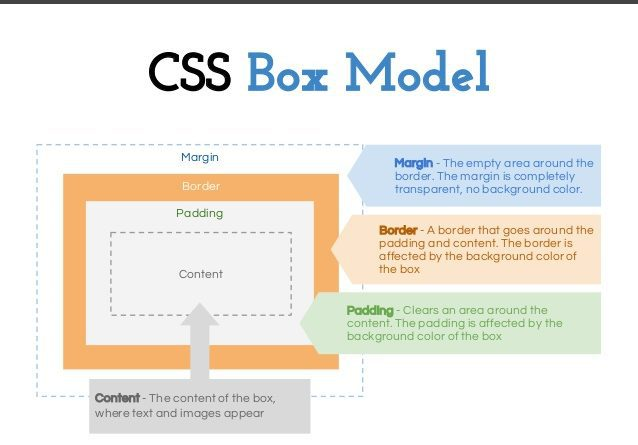
\includegraphics[scale=0.5]{css-box-model}
\end{frame}


\begin{frame}{CSS pozicování}
	  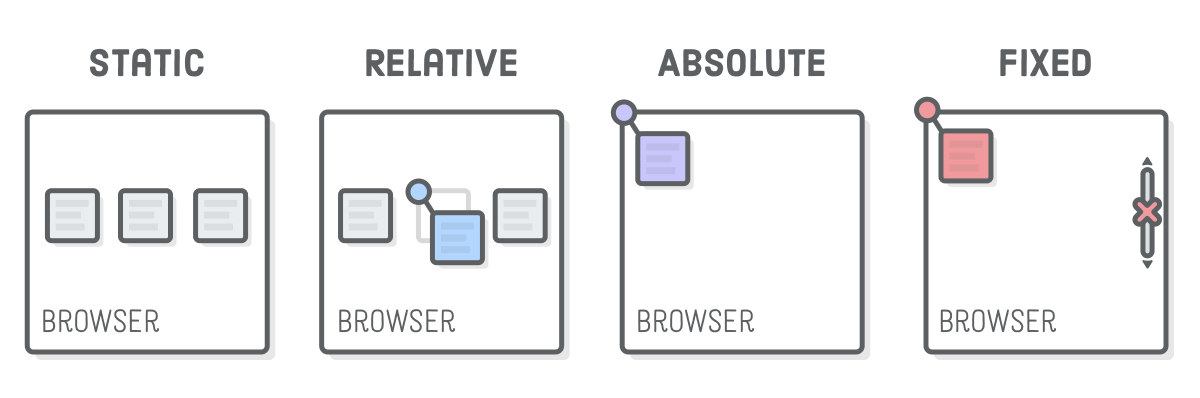
\includegraphics[scale=0.26]{css-positioning}
	\begin{itemize}
		\item \url{https://www.w3schools.com/cssref/pr_class_position.asp}
		\item \url{https://internetingishard.com/html-and-css/advanced-positioning/}
	\end{itemize}
\end{frame}

\begin{frame}{CSS obtékání}
	  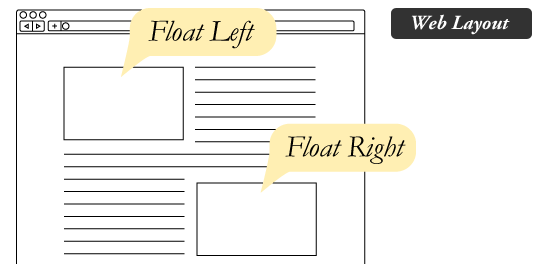
\includegraphics[scale=0.5]{css-floating}
	\begin{itemize}
		\item \url{https://css-tricks.com/all-about-floats/}
		\item \url{https://w3schools.com/css/css_float.asp}
	\end{itemize}
\end{frame}


\begin{frame}{CSS layout -- flexbox}
	  
\includegraphics[scale=0.5]{css-flexbox}
	\begin{itemize}
		\item \url{https://w3schools.com/css/css3_flexbox.asp}
		\item \url{https://css-tricks.com/snippets/css/a-guide-to-flexbox/}
	\end{itemize}
\end{frame}

\begin{frame}{CSS layout -- grid}
	  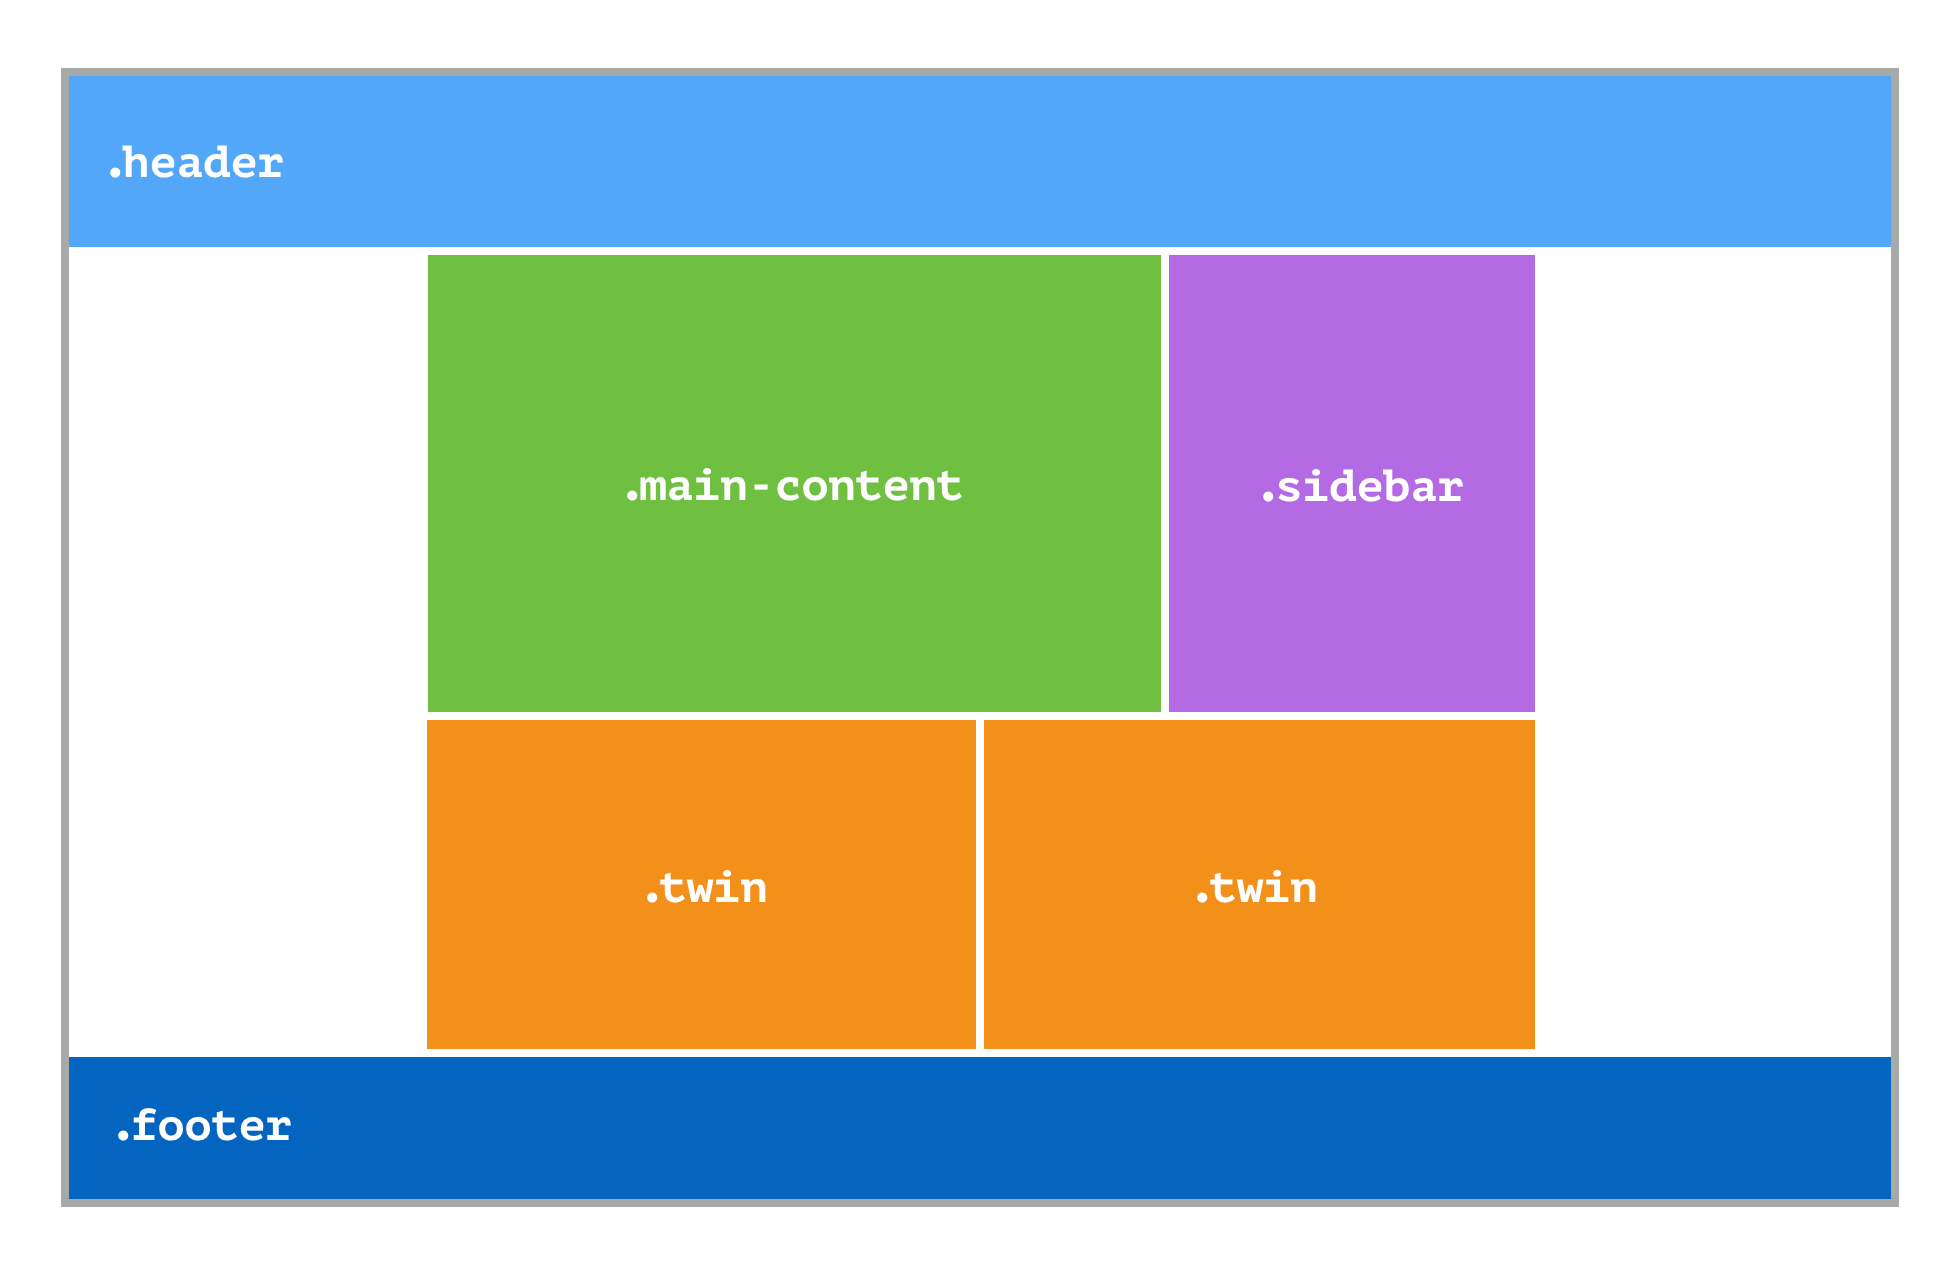
\includegraphics[scale=0.15]{css-grid}
	\begin{itemize}
		\item \url{https://w3schools.com/css/css_grid.asp}
	\end{itemize}
\end{frame}


\begin{frame}[fragile, shrink=0]{@ pravidla}
  \begin{itemize}
	\item "at" pravidla jsou speciální příkazy
\end{itemize} 

\begin{itemize}
	\item \textbf{@import} -- import stylu
\end{itemize}
\begin{lstlisting}[language=HTML]
@import url(style.css);
\end{lstlisting}

\begin{itemize}
	\item \textbf{@media} -- svazuje styly s konkrétním typem výstupu
\end{itemize}
\begin{lstlisting}[language=HTML]
@media only screen and (max-width: 600px) {
/*vlastnosti pro nizke rozliseni*/}
@media print {/* vlastnosti pro tisk */} 
\end{lstlisting}

\begin{itemize}
	\item \textbf{@font-face} -- import vlastních fontů
\end{itemize}
\begin{lstlisting}[language=HTML]
@font-face {font-family: "Scarborough Light"; 
src: url("http://www.font.site/s/scarbo-lt");}
\end{lstlisting}
\end{frame}

\begin{frame}[fragile, shrink=0]{@ pravidla -- ukázka pro tisk}
\begin{itemize}
	\item příklad použití
\end{itemize} 


\begin{lstlisting}[language=HTML]
@media print {
    body {
        color: #000;
        background: #fff;
    }
}
\end{lstlisting}


\end{frame}


\begin{frame}[fragile, shrink=0]{Viewport}
\begin{itemize}
	\item viditelná oblast stránky
	\item zaleží na zařízení (desktop, telefon)
\end{itemize} 

 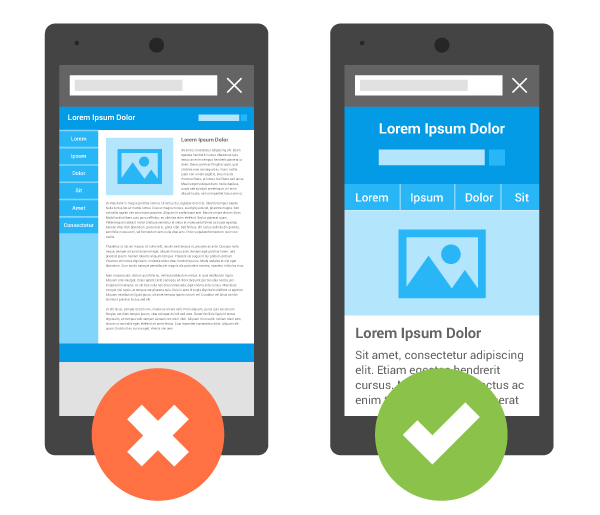
\includegraphics[scale=0.3]{viewport}


\begin{lstlisting}[language=HTML]
<meta name="viewport" 
content="width=device-width, initial-scale=1">
\end{lstlisting}
\begin{itemize}
	\item dojde k přepočtu pixelů
	\item telefony mají vysoké rozlišení, ale malý displej
	\item \url{www.vzhurudolu.cz/prirucka/viewport}
\end{itemize}

\end{frame}



\begin{frame}{Kontrolní otázky}
\begin{itemize}
	\item Co znamená akronym CSS?
	\item Co je to selektor?
	\item Jaké máme v CSS délkové jednotky?
	\item Jaký je rozdíl mezi řádkovými a blokovými elementy?
	\item Jakou vlastností můžeme změnit blokový element na řádkový element?
	\item Co jsou to plovoucí elementy?
	\item Jaké máme formy pozicování elementů?
	\item Co jsou to @ pravidla?
	\item jak je možné řídit vykreslování překrývajících se elementů?  
\end{itemize}
	
\end{frame}



\begin{frame}[fragile, shrink=0]{Bootstrap}
\begin{itemize}
	\item CSS framework pro responsivní web design
	\item \url{https://www.w3schools.com/bootstrap4/}
	\item \url{https://mobirise.com/_l/bootstrap-website-builder/}
\end{itemize}

\end{frame}
	  

\end{document}